\documentclass{beamer}
%\usepackage{colortbl}
\usepackage[latin1]{inputenc}
\usepackage{comment}
%\usetheme{Warsaw}
\usetheme{Frankfurt}
%\usecolortheme{dove}
\usefonttheme{serif} 

\usepackage[absolute,overlay]{textpos} 
\usepackage{booktabs}
\usepackage{color}
\usepackage{threeparttable}
\usepackage{multirow}
%\usepackage[table]{xcolor}
%\definecolor{tableShade}{HTML}{F1F5FA}
\usepackage[normalem]{ulem}


\title[Epistasis in GWAS]{2D or not 2D, that is the question\\
{\footnotesize Should we be looking for epistasis in GWAS?}}
\author{Gibran Hemani}
\institute{The Roslin Institute, University of Edinburgh \\
\vspace{.3cm}
Diamantina Institute \\and \\
Queensland Brain Institute,\\
University of Queensland}
\date{}
\begin{document}

\AtBeginSection[]
{
  \begin{frame}<beamer>
    \frametitle{Outline}
    \tableofcontents[currentsection,currentsubsection]
  \end{frame}
}

\begin{frame}
\titlepage
\end{frame}

\begin{comment}


____________intro

talk about gwas design from an evolutionary perspective
- interesting paradox in quan genetic theory

what is a gwas?
mixed success. missing heritability

additive genetic variance paradigm
- additive effects
- heritability estimates (problems with mz and dz twin studies? occam's razor?)
- fitness vs morphological traits (response to selection, maintenance of additive variance)

epistasis
- define epistasis
- how to search (two stages, two dimensions, mention epiGPU)

can epistasis maintain additive variance?
- yes.
- it actually maintains non-additive variation much more
- how do we search for epistasis?

____________conclusions

is the observation of additive variance an illusion?
have we misused occam's razor?
here is the paradox:
if you can measure additive genetic variance, search for non-additive variance

____________acknowledgements


\end{comment}

\begin{frame}{}
\begin{itemize}
\item \textbf{Simulations:} An evolutionary perspective on genetic variation
\item \textbf{Computation:} Making epistatic searches possible
\item \textbf{Thresholds:} What should we call `significant'?
\item \textbf{Data:} What do we find empirically?
\end{itemize}
\end{frame}

\section{Evolutionary simulations}
\subsection{}

\begin{frame}{Epistasis}
\begin{definition}
{\color{orange} The effect on the phenotype caused by locus A depends on the genotype at locus B }
%{\tiny \color{white} \newline - Carlborg and Haley 2004 }
\end{definition}
\end{frame}

\begin{frame}{Epistasis and additive variance}
\begin{center}
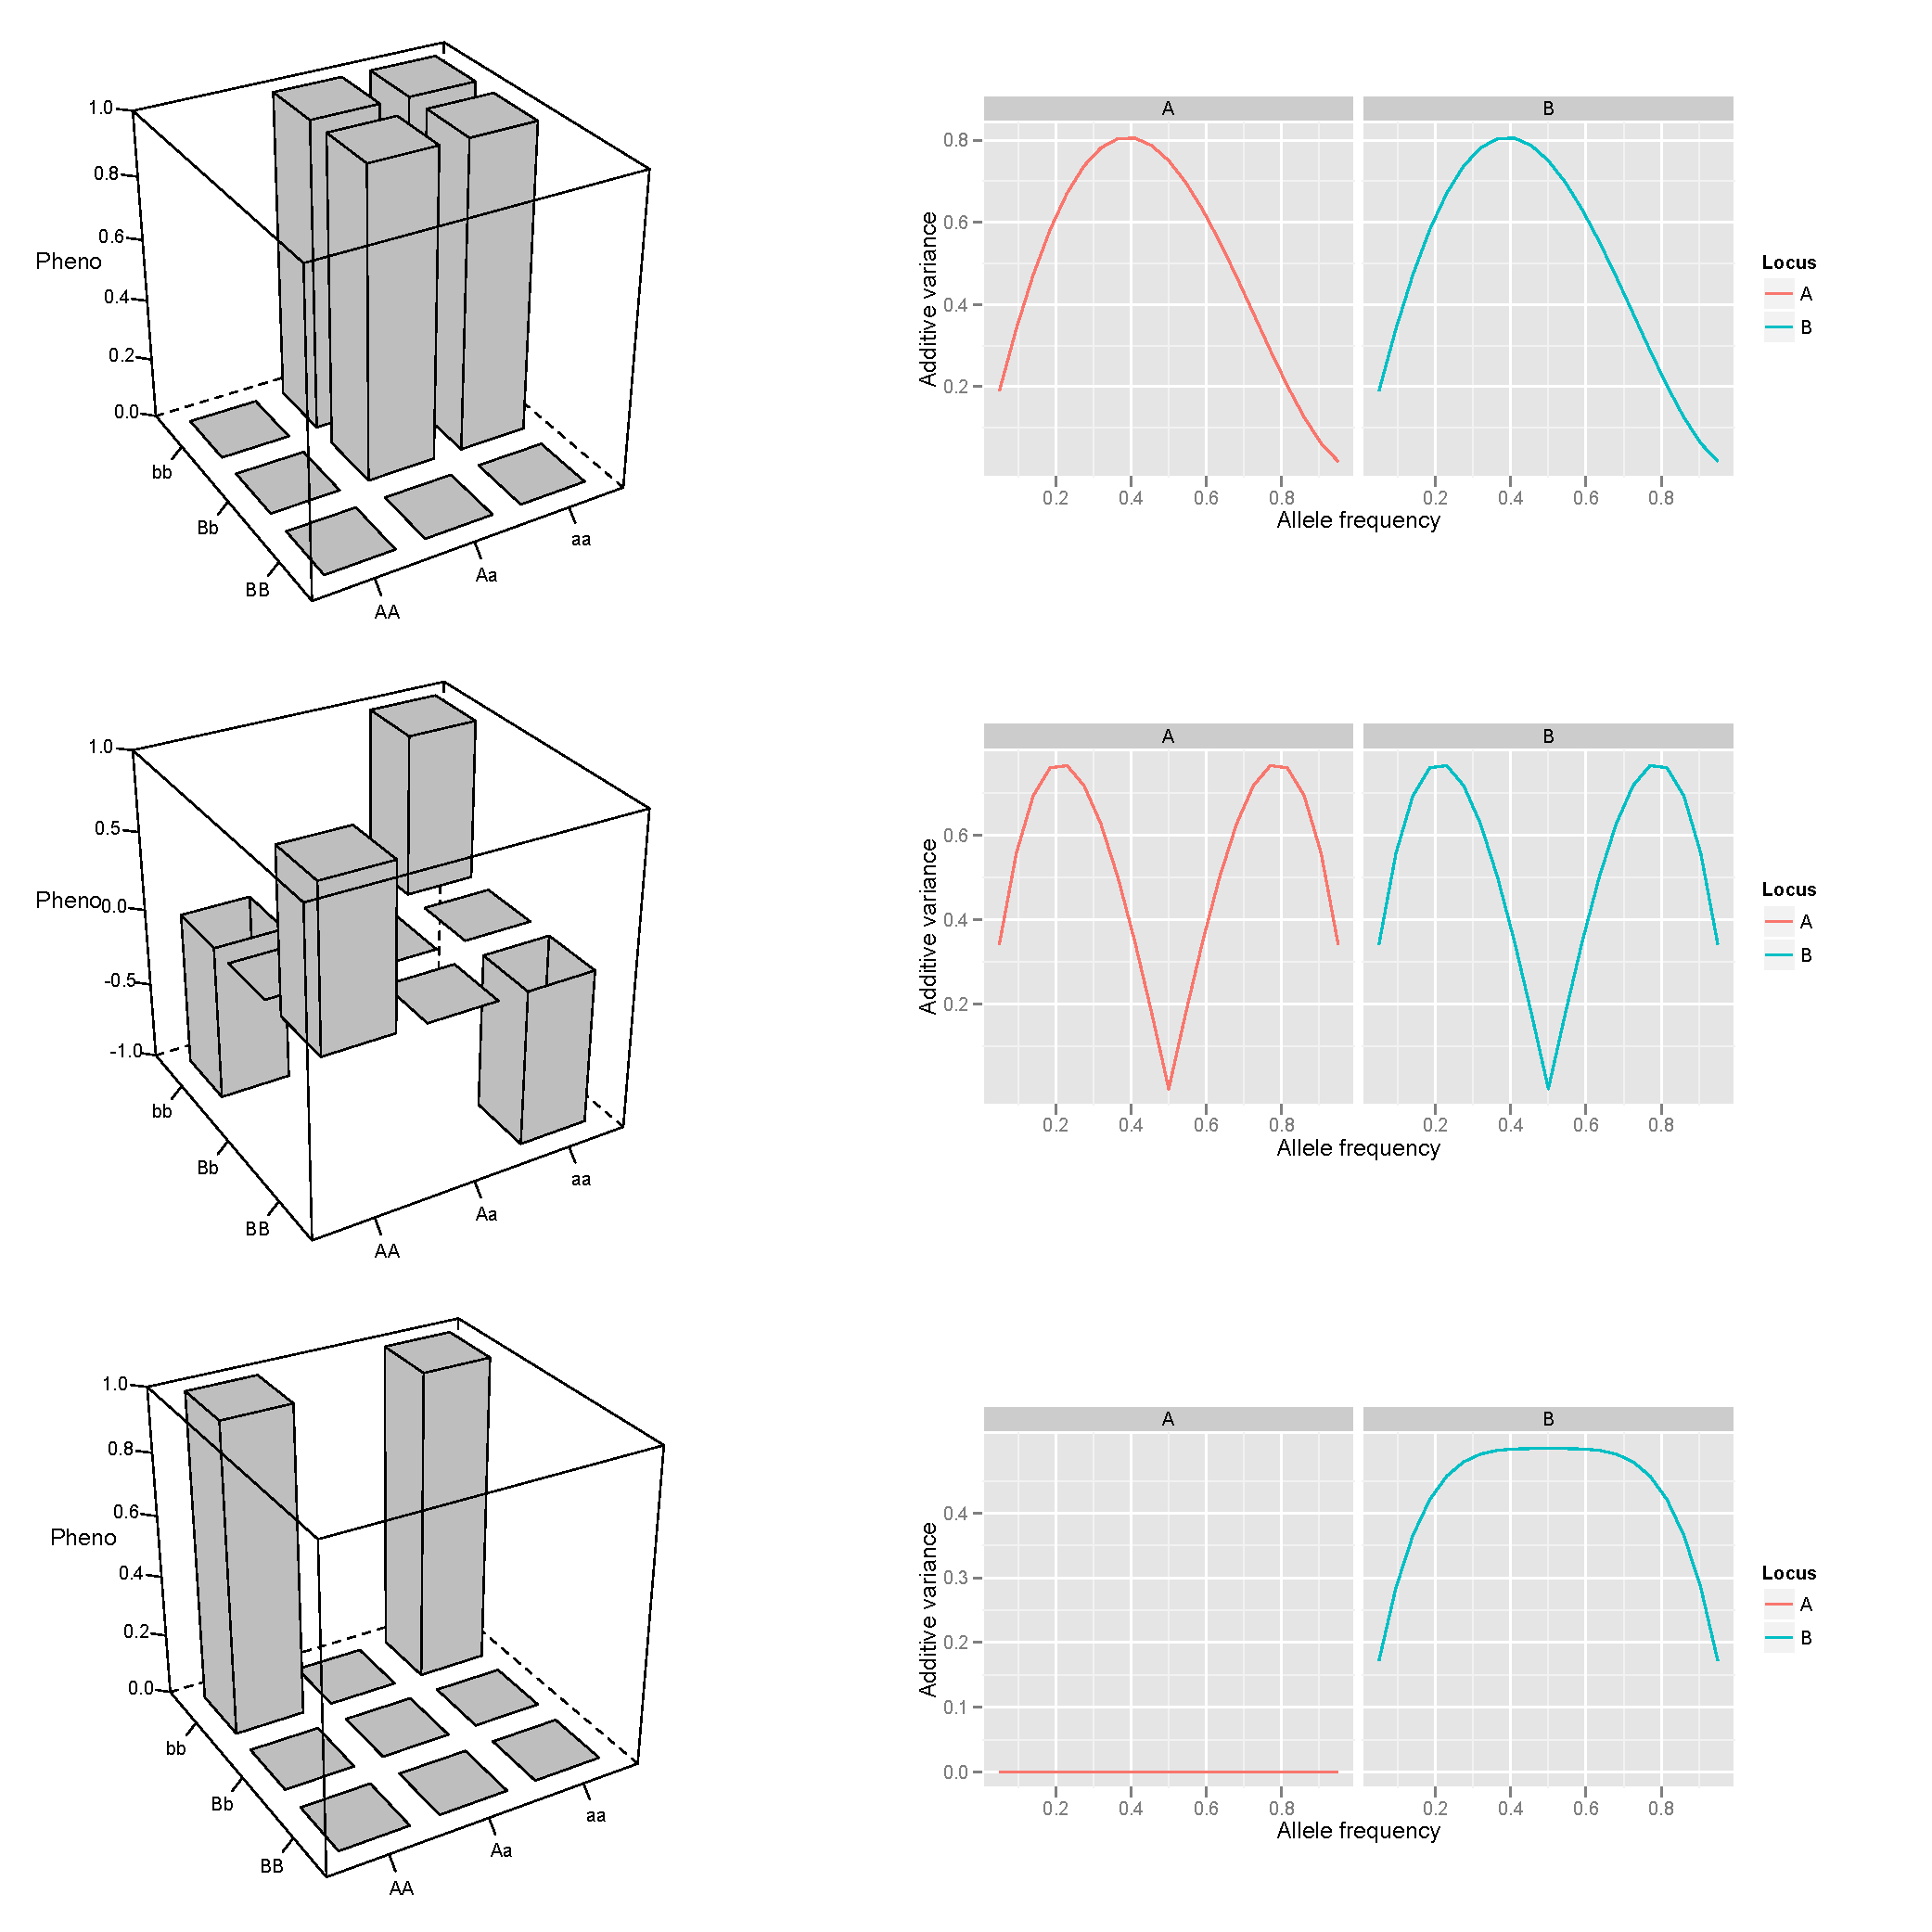
\includegraphics[height=7cm]{gp_va}
\end{center}
\end{frame}

\begin{frame}{}
\textbf{Hypothesis:}\\ Epistasis can maintain additive variance better than purely additive effects
\end{frame}


\begin{frame}{Epistasis maintains genetic variation}
\begin{center}
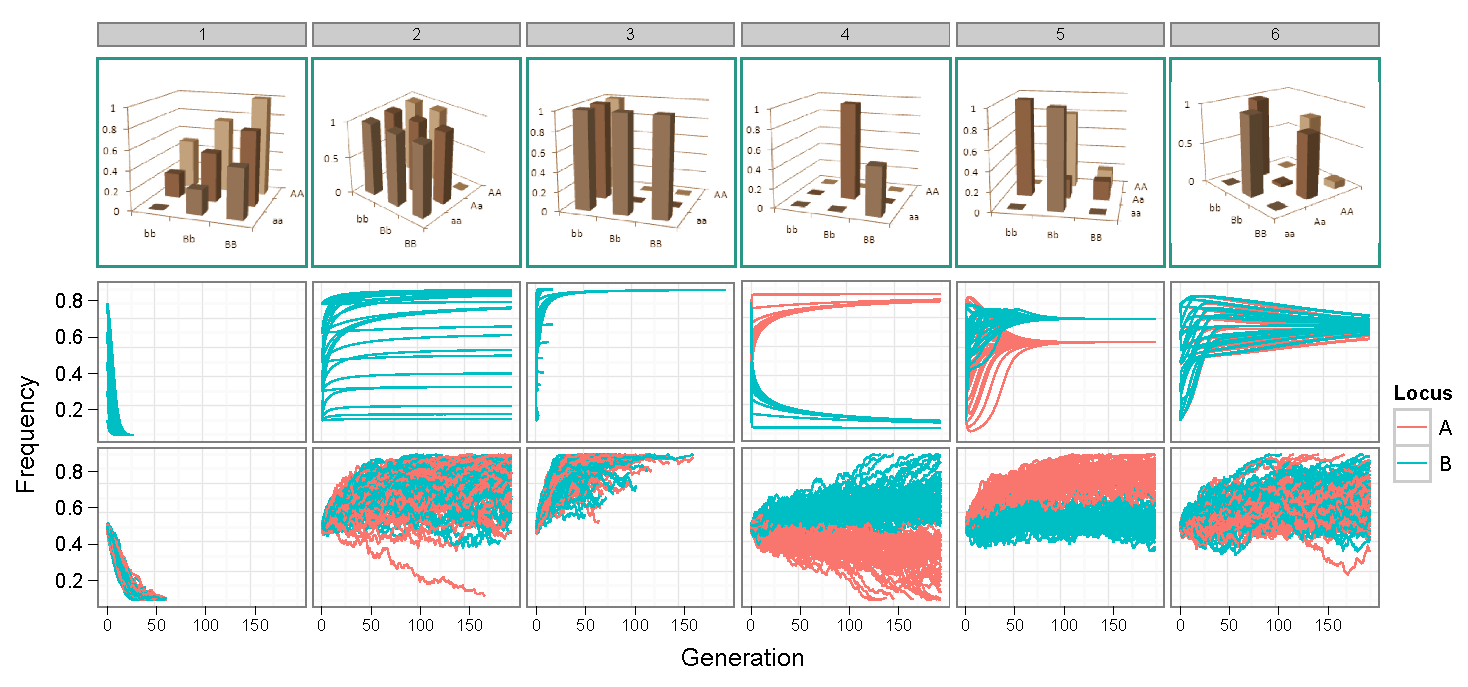
\includegraphics[width=11cm]{maps_freqs}
\end{center}
\end{frame}

\begin{frame}{Most of the variance is non-additive}
\begin{center}
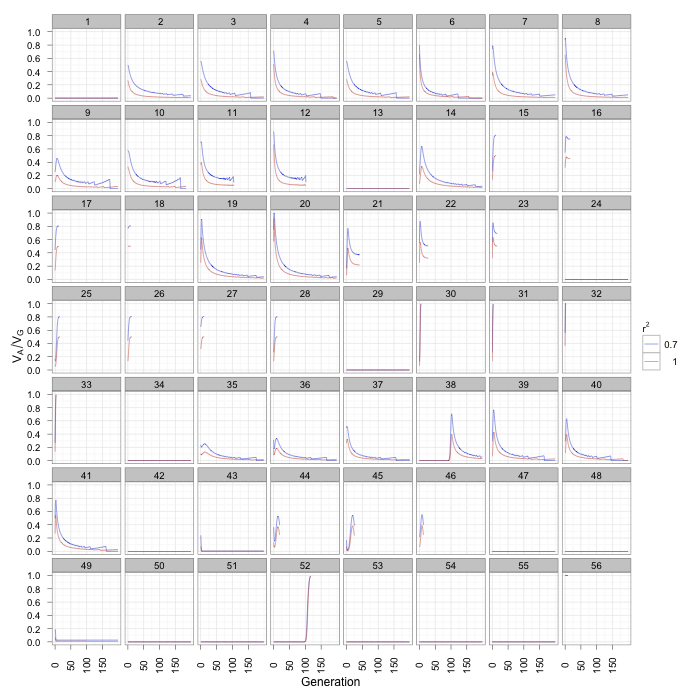
\includegraphics[width=8cm]{sup_propadditive_det.png}
\end{center}
\end{frame}

\begin{frame}{Impact of LD on observed variance}
\begin{center}
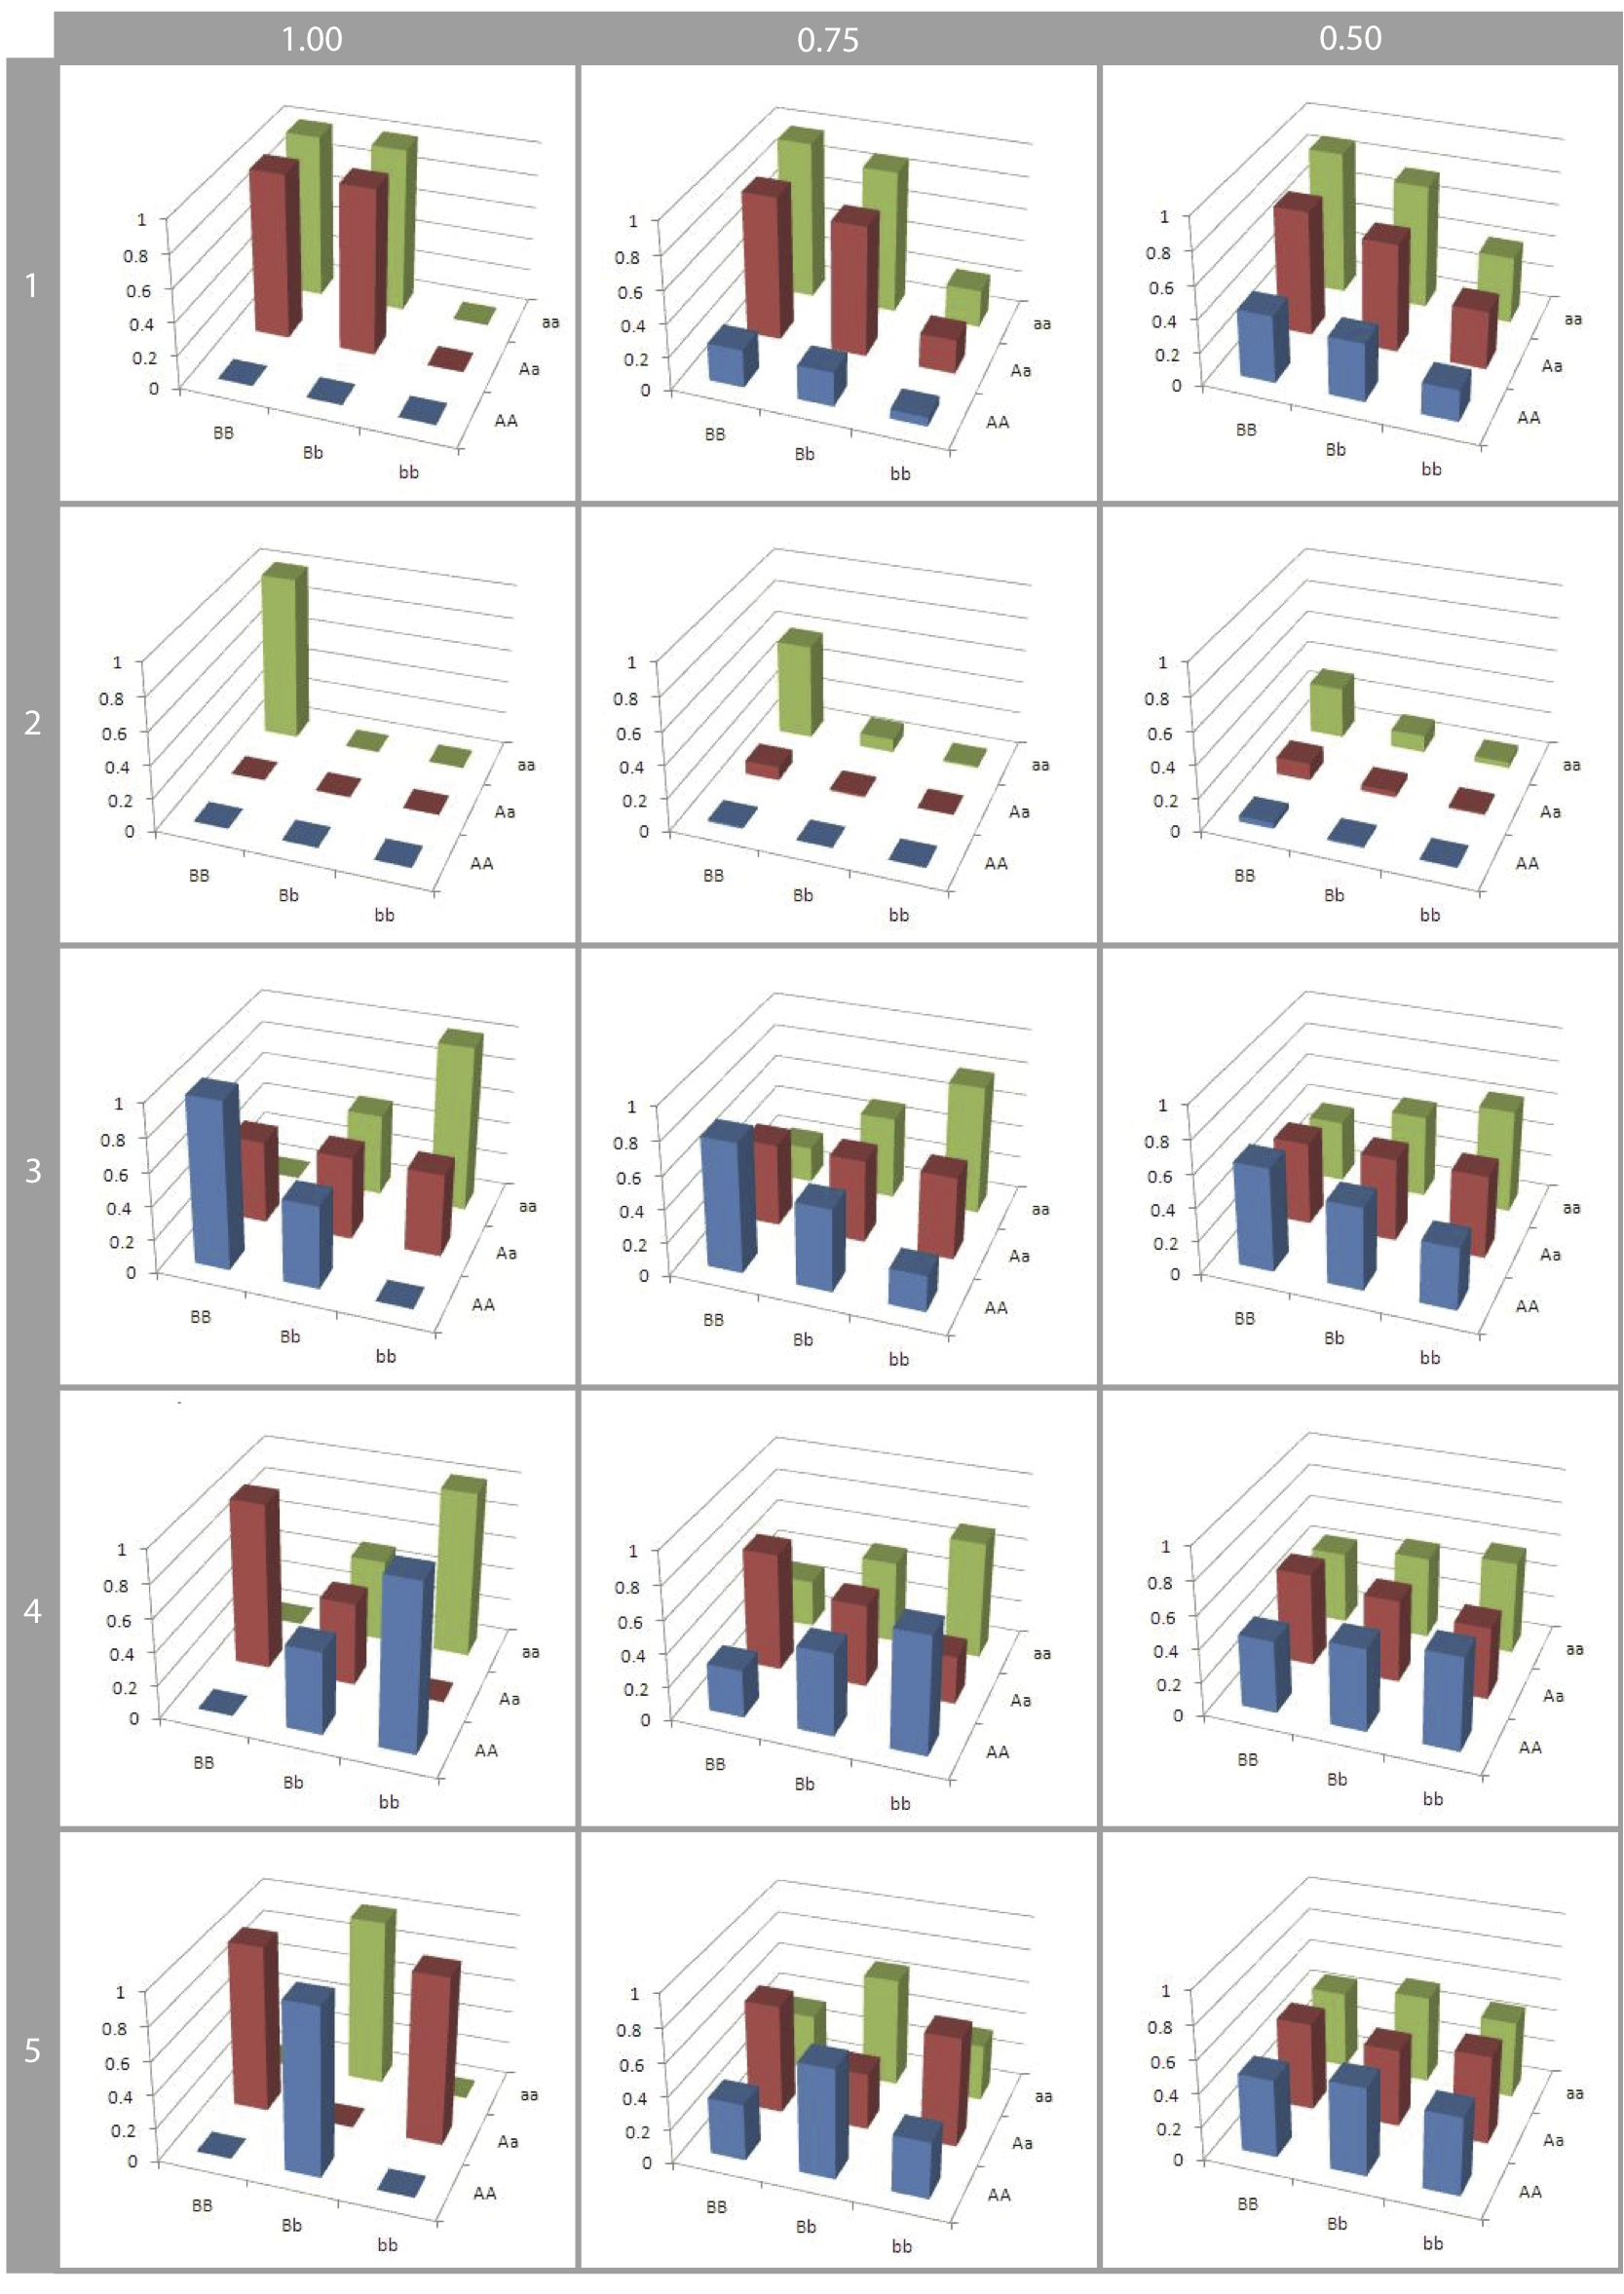
\includegraphics[width=5cm]{gpmaps_ld.png} \\
\end{center}
\end{frame}


\begin{frame}{With high LD, 2D searches are most powerful}
\begin{columns}[c]
\column{.7\textwidth}
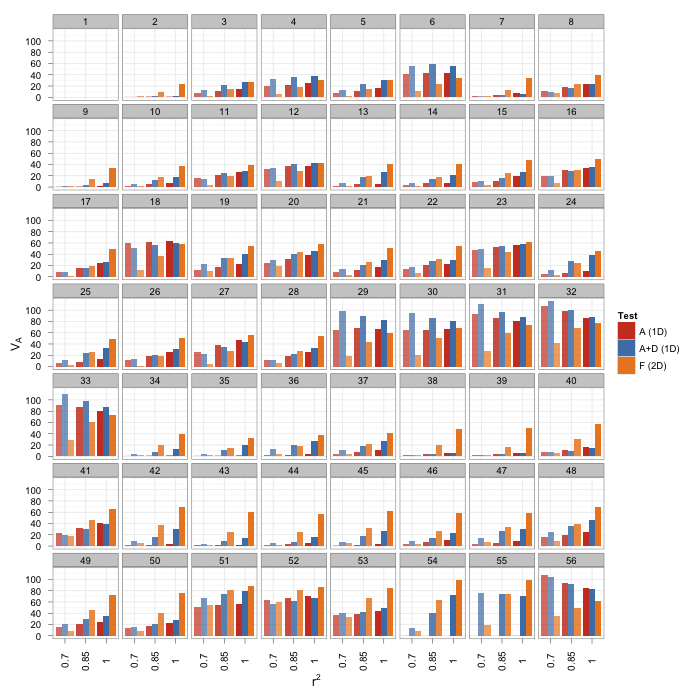
\includegraphics[width=8cm]{sup_heritbars_sim.png}
\column{.3\textwidth}
When LD between causal variants and observed SNPs is high, 2D scan is most powerful for 46/54 non-additive patterns
\end{columns}
\end{frame}

\begin{frame}{The paradox}
\begin{columns}[c]
\column{.5\textwidth}
\begin{itemize}
\item Epistasis can contribute towards the maintenance and observation of additive genetic variance
\item To find the missing additive variance, search for epistatic effects
\end{itemize}
\column{.5\textwidth} 
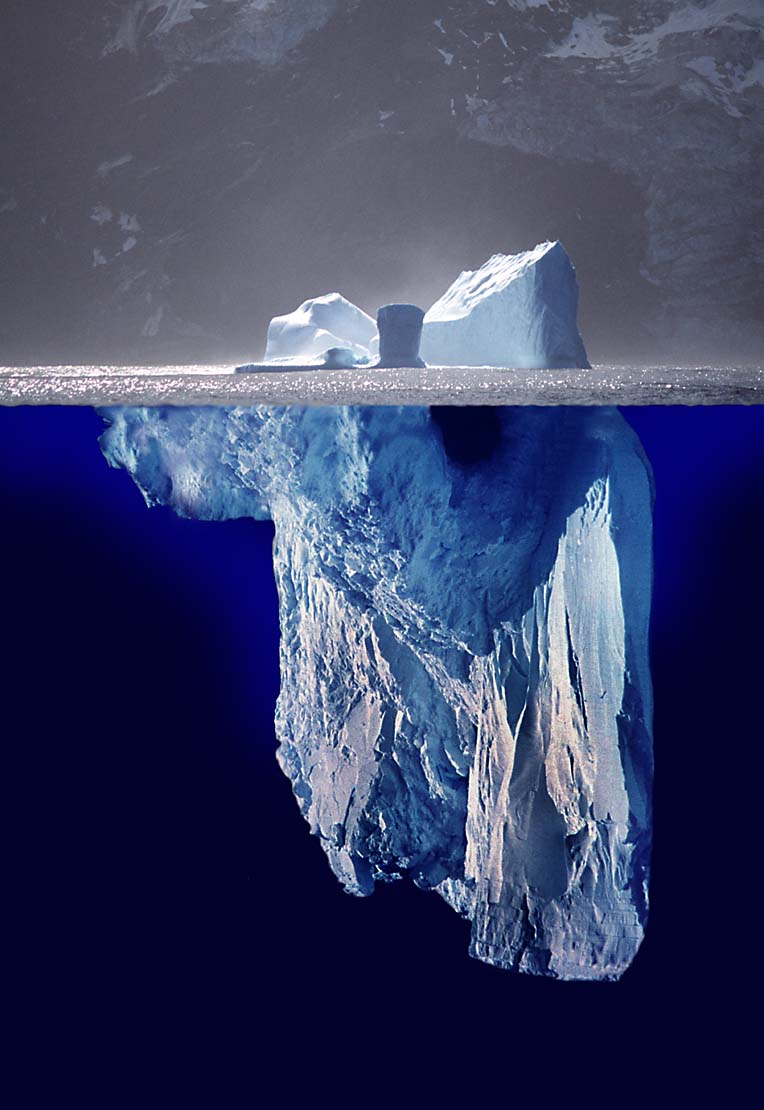
\includegraphics[height=6.5cm]{iceberg.jpg} \\
\end{columns}
\end{frame}


\section{Computational solutions}
\subsection{}

\begin{frame}{The problem}
Number of interactions: \\
\begin{equation}
n(n-1) / 2 \nonumber
\end{equation}
500000 SNPs $\rightarrow$ 125 billion interactions \\
\begin{itemize}
\item For 1000 individuals, PLINK performs 5000 tests per second $\rightarrow$ 3 years
\item FastEpistasis performs 36000 tests per second $\rightarrow$ 5 months
\item Optimised C code 125000 tests per second $\rightarrow$ 6 weeks
\item Parallelised on 8-core CPU $\rightarrow$ 5 days
\end{itemize}
\end{frame}


\begin{frame}{CPU limits}
\begin{center}
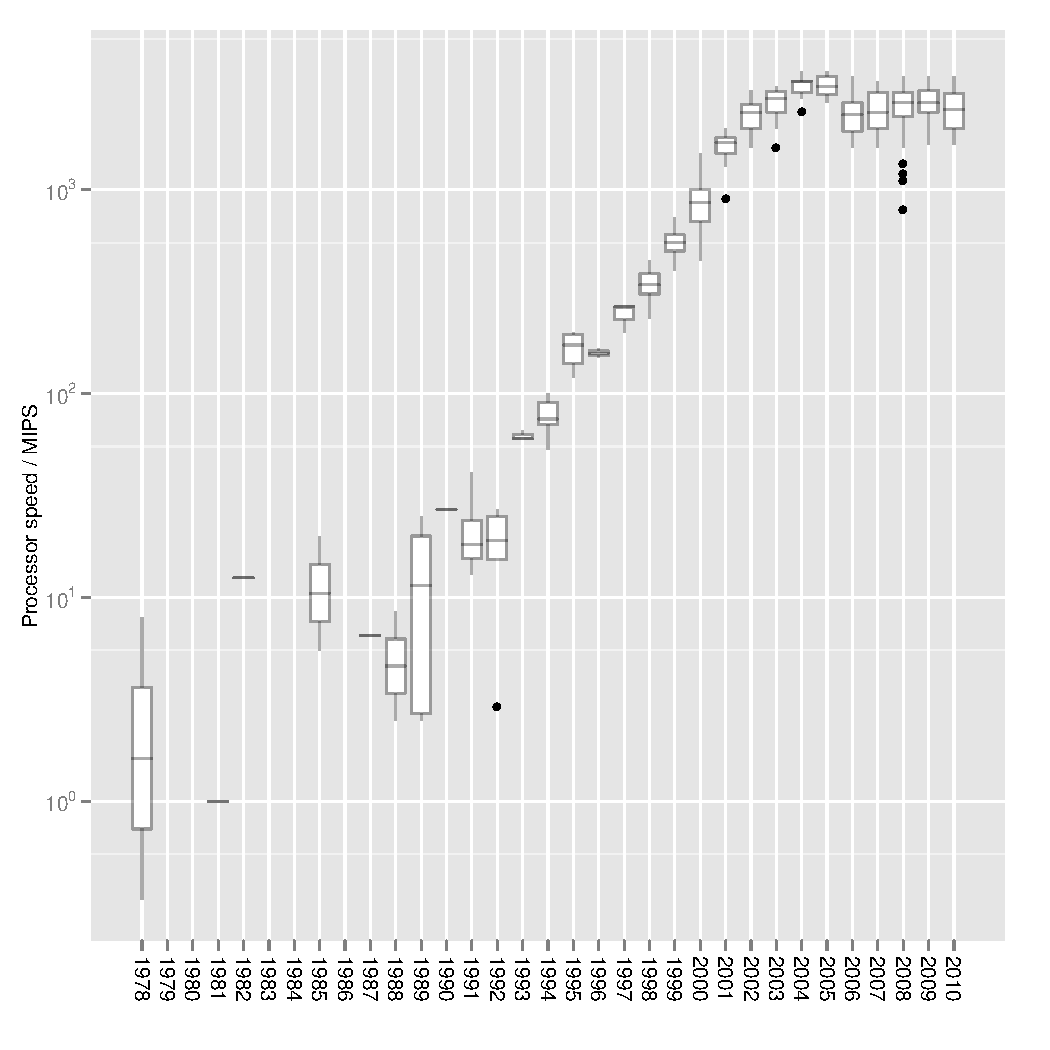
\includegraphics[height=7cm]{clockspeed.pdf}
\end{center}
\end{frame}


\begin{frame}{Graphics Cards}
\begin{center}
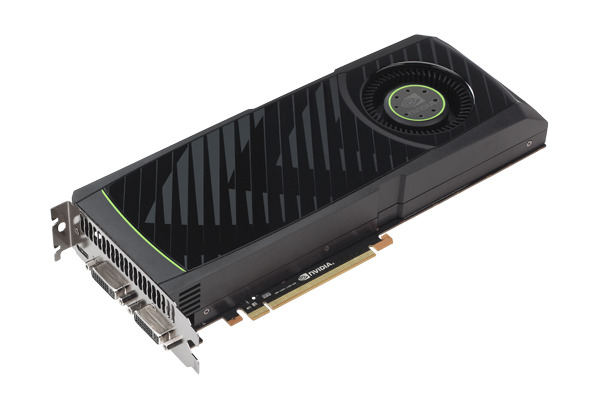
\includegraphics[width=10cm]{gtx580}
\end{center}
\end{frame}



\begin{frame}{GPU speeds}
\begin{center}
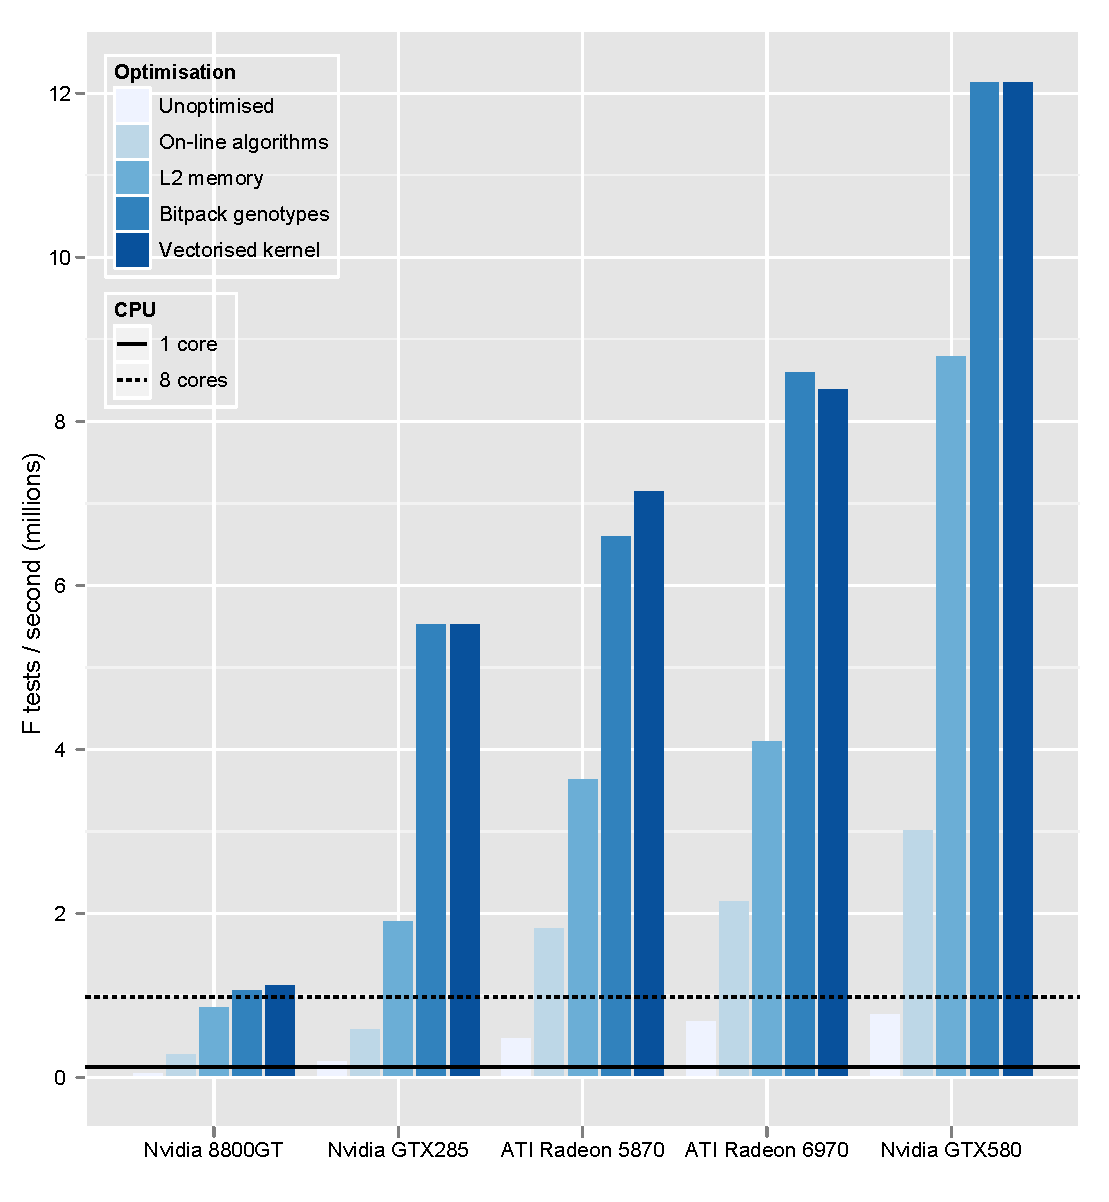
\includegraphics[height=7cm]{gpuoptimisation.pdf}
\end{center}
\end{frame}

\begin{frame}{epiGPU}
\begin{itemize}
\item http://sourceforge.net/projects/epigpu/
\item Free
\item Open source
\item Windows, Mac, Linux
\item NVIDIA and ATI graphics cards
\end{itemize}
\end{frame}


\begin{frame}{Other optimised epistasis software}
\begin{itemize}
\item BiForce
\item GLIDE
\item GBOOST
\item TEAM
\item MDR-GPU
\item EPIBLASTER
\item SHEsisEPI
\item ...probably more
\end{itemize}
\end{frame}


\section{Thresholds}
\subsection{}

\begin{frame}{The curse of dimensionality}
As the dimensionality of the search increases the background noise drowns out all real biological signals
\end{frame}

\begin{frame}{Linkage disequilibrium}
\begin{center}
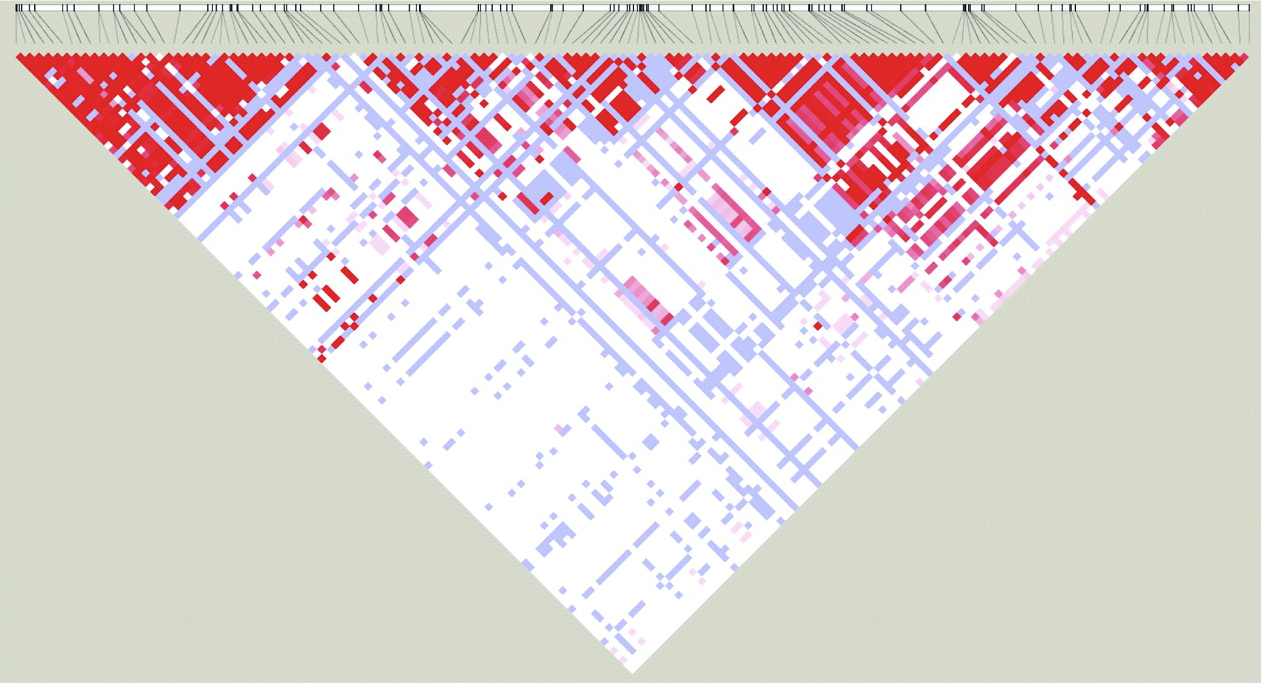
\includegraphics[width=10cm]{ld.png}
\end{center}
\begin{itemize}
\item SNPs are correlated $\rightarrow$ tests are not independent
\item Bonferroni correction is overly stringent
\item What is the correlation structure in a 2D search?
\end{itemize}
\end{frame}


\begin{frame}{Permutation analysis}
What is the \emph{effective} number of multiple tests that are being performed? (Churchill 1994)
\begin{center}
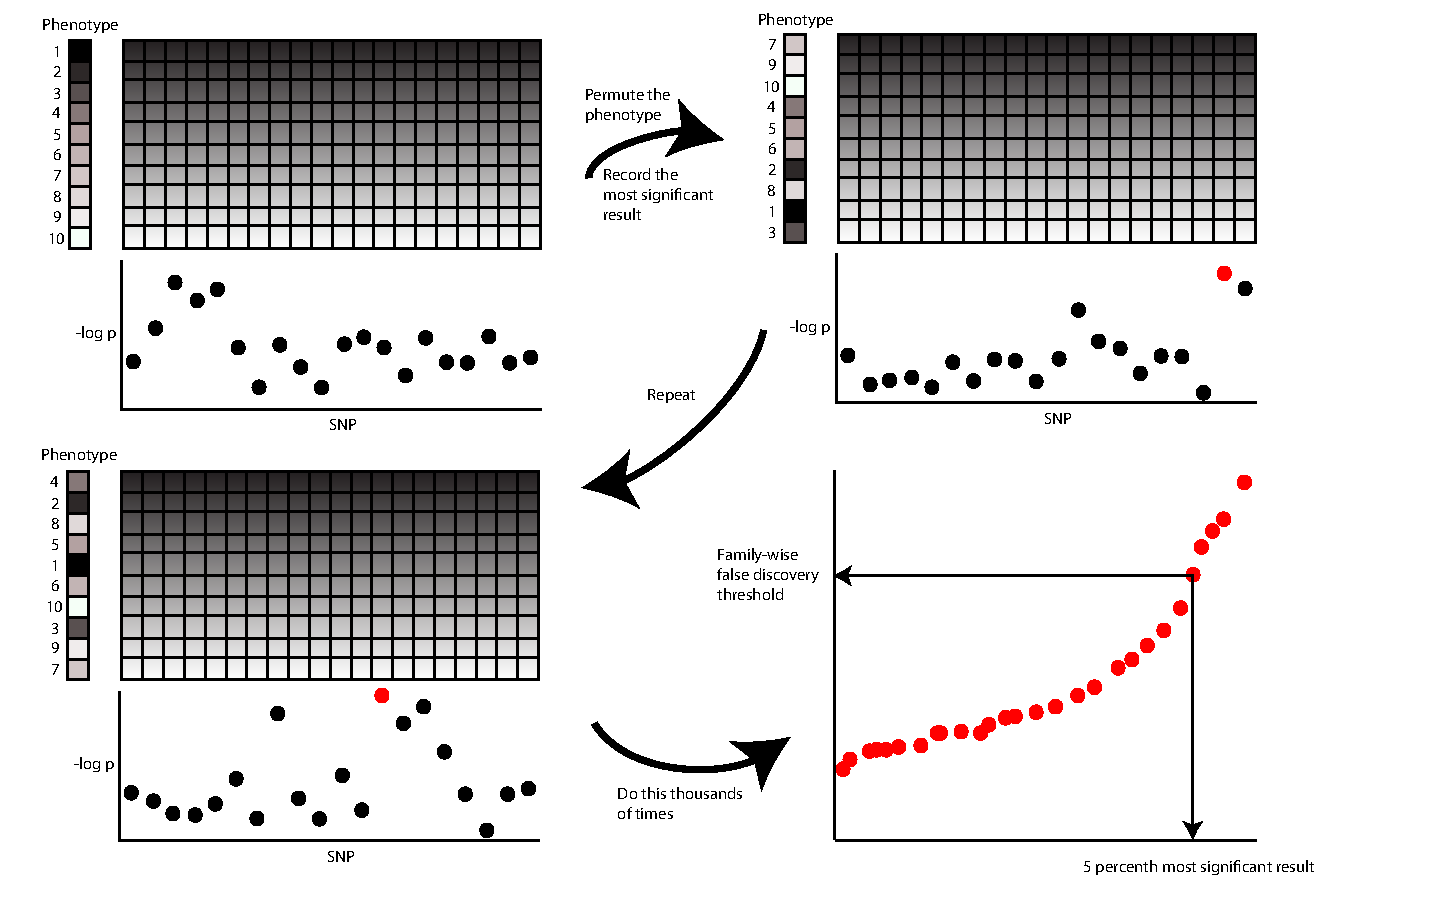
\includegraphics[width=10cm]{permutationanalysis.pdf}
\end{center}
\end{frame}


\begin{frame}{A general formula for 2D thresholds?}
\begin{equation}
-\log_{10}(p_{T}) = a - \frac{a}{f_{1}(N)+ f_{2}(M)} \nonumber
\label{eqn:general_threshold}
\end{equation}
\begin{eqnarray}
a & = & -\log_{10} \left (\frac{0.05}{t^2/2} \right) = 12.68 \nonumber
\end{eqnarray}
where $t = 693138$ is the number of independent regions in the genome (Dudbridge \& Gusnanto 2008)
\end{frame}

\begin{frame}{A general formula for 2D thresholds?}
\begin{center}
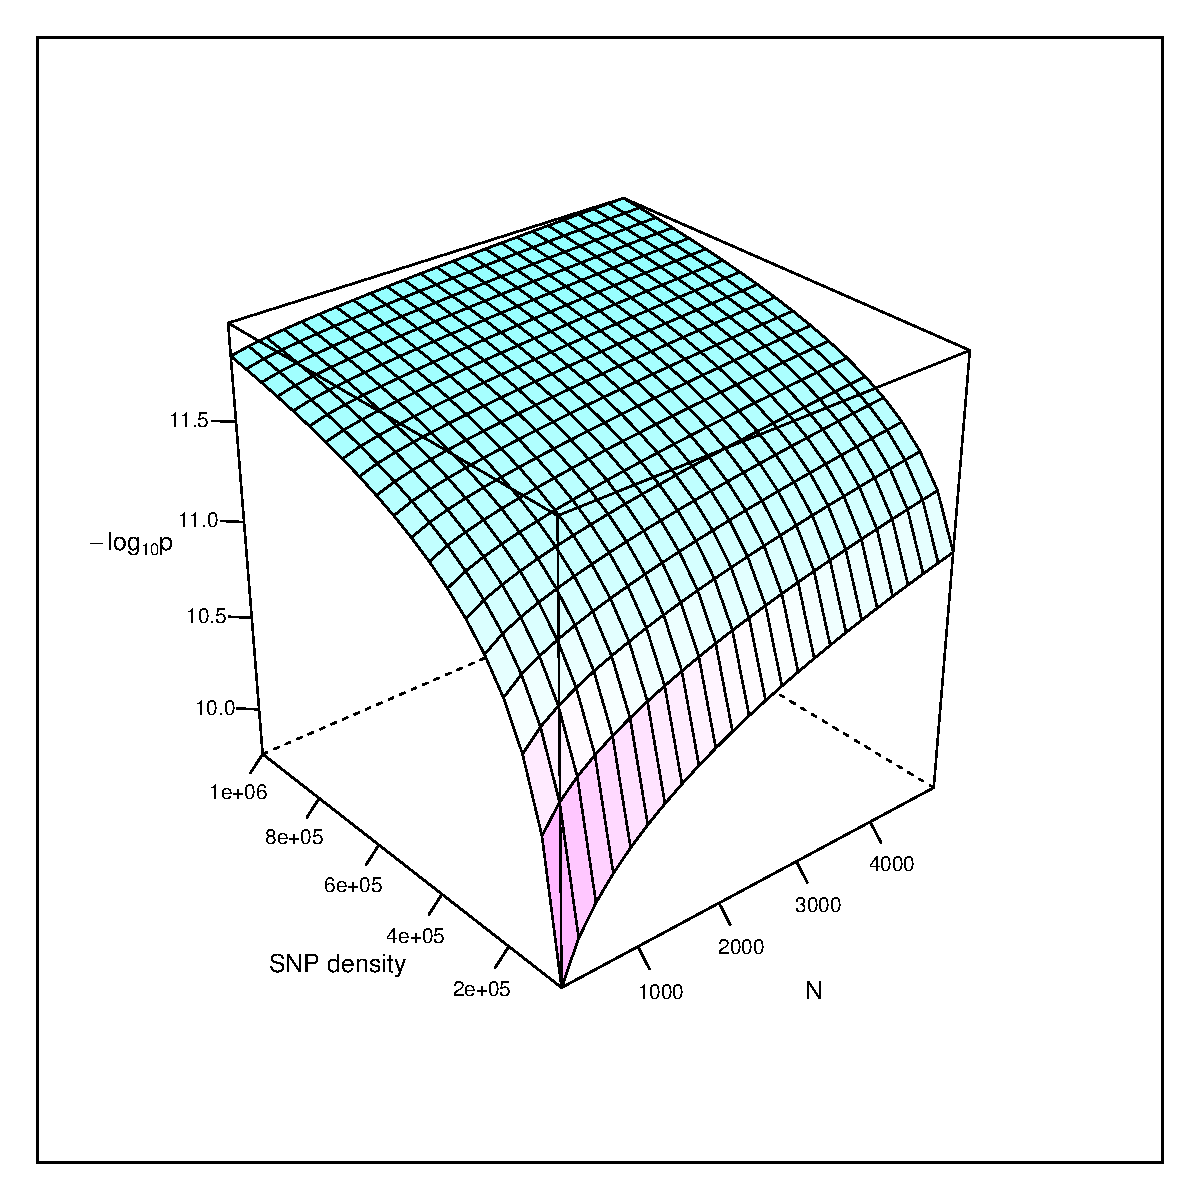
\includegraphics[height=7cm]{threshold_function.pdf}
\end{center}
\end{frame}


\section{2D eQTL}
\subsection{}

\begin{frame}{Are epistatic effects controlling gene expression?}
\begin{itemize}
\item Study design:
\begin{itemize}
\item 846 healthy Australian adults
\item 546,192 SNPs
\item 5380 gene expression probes from whole blood
\end{itemize}
\item Plan:
\begin{itemize}
\item Do exhaustive search for 2 locus epistasis for each probe
\item Parallelise search across 100x GPU cluster
\end{itemize}
\end{itemize}
\end{frame}

\begin{frame}{Thresholds}
\begin{itemize}
\item 1641 complete scans were performed on permuted phenotype
\item Threshold predicted to be: \textbf{11.648}
\item Empirical estimate: \textbf{11.632}
\item Average correlation between 5380 probes: \textbf{0.265}
\item Overall threshold: $-\log_{10}p =$ \textbf{16.5}
\end{itemize}
\end{frame}

\begin{frame}{Very preliminary results}
\begin{itemize}
\item Is there much non-additive variance?
\item 71 probes have significant eQTLs after filtering for:
\begin{itemize}
\item Threshold of 16.5
\item Additive variance $\leq$ 60\% of total genetic variance
\item Relatively common SNPs (must have samples for all 9 genotype classes)
\item No LD between interacting SNPs
\end{itemize}
\item Total of 140 significant independent loci
\end{itemize}
\end{frame}

\begin{frame}{Very preliminary results}
\begin{itemize}
\item Proportion of the phenotypic variance explained:
\begin{itemize}
\item Total genetic: range 8.4\% - 17.1\%
\item Total non-additive: range 3.5\% - 9.2\%
\end{itemize}
\item 14\% cis-cis
\item 69\% cis-trans
\item 17\% trans-trans
\end{itemize}
\end{frame}

\begin{frame}{Some examples}
\begin{center}
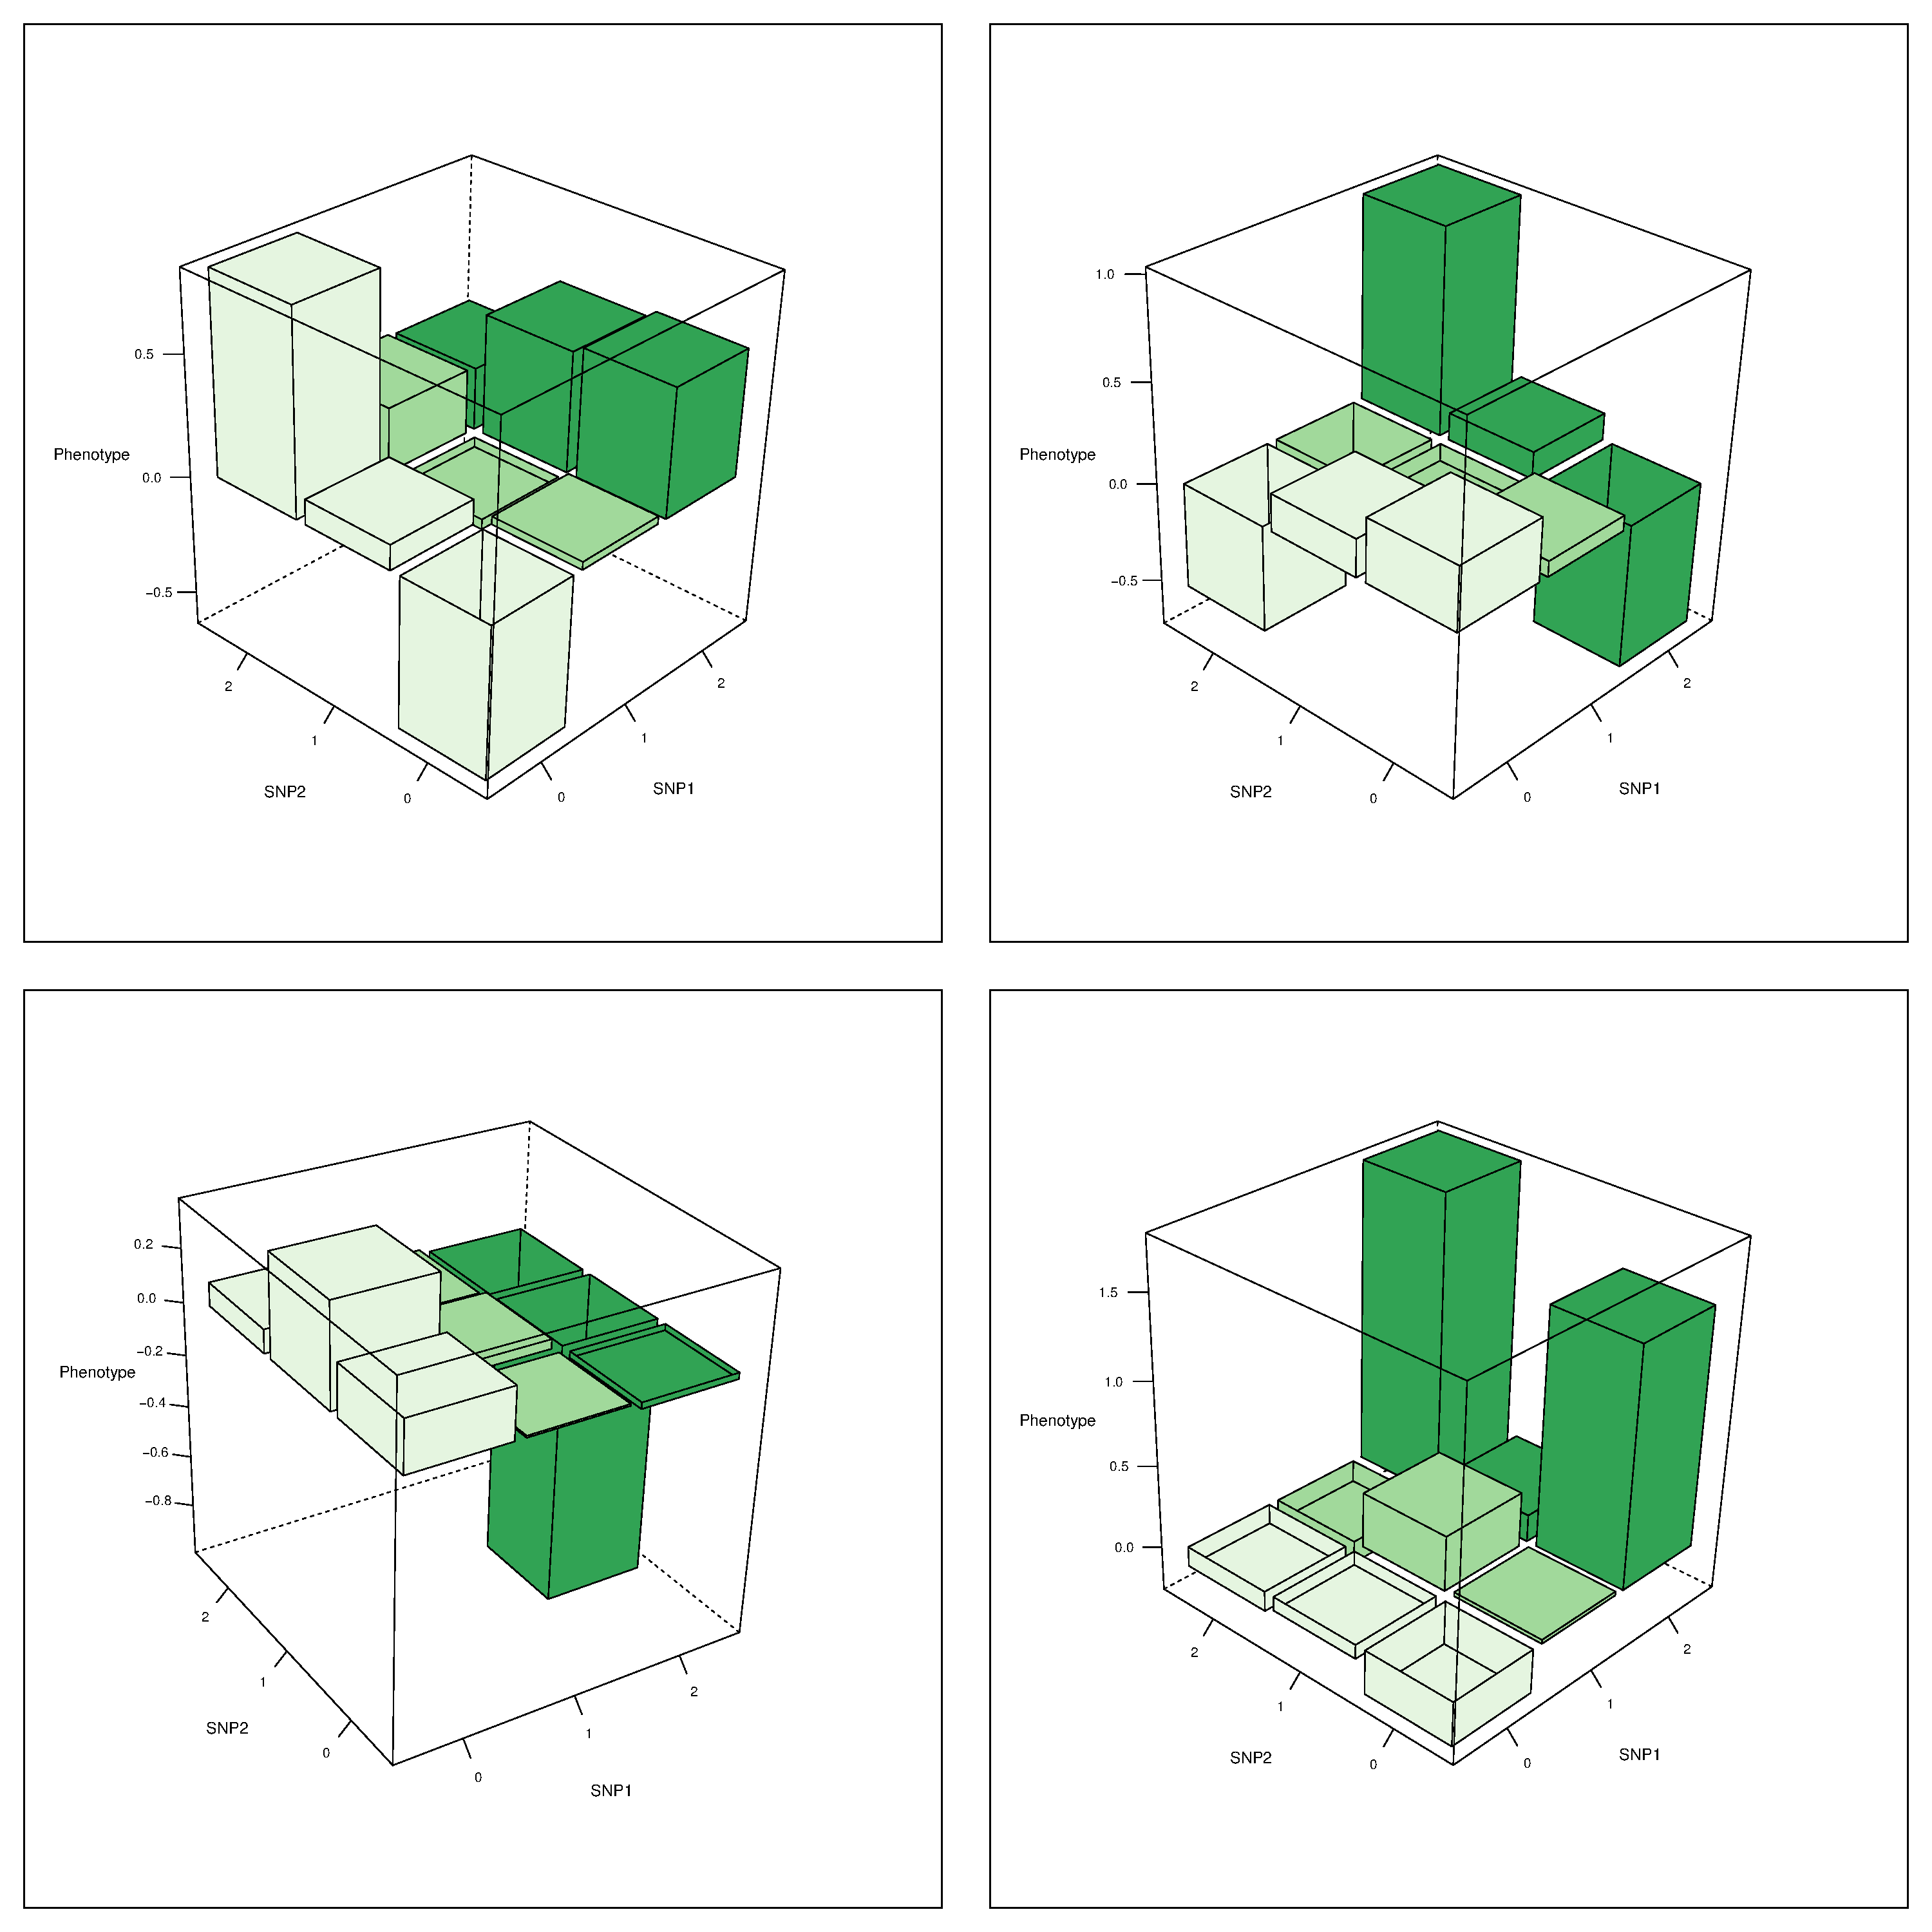
\includegraphics[height=7.5cm]{epistasis_examples}
\end{center}
\end{frame}


\section*{}

\begin{frame}{Acknowledgements}


\begin{columns}[c]

\column{.5\textwidth}

{\tiny
PhD Funding:
\begin{itemize}
\item The Roslin Institute
\item University of Edinburgh
\item Biosciences KTN
\item Monsanto / Newsham Choice Genetics
\end{itemize}
PhD Supervisors:
\begin{itemize}
\item Chris Haley
\item Sara Knott
\item John Woolliams
\end{itemize}
Important people:
\begin{itemize}
\item Ricardo Pong-Wong
\item Athanasios Theocharidis
\item Wenhua Wei
\end{itemize}
Compute resources
\begin{itemize}
\item ECDF - {\tt eddie}
\item Daresbury Labs - {\tt cseht}
\item IVEC - {\tt fornax}
\item QBI cluster
\end{itemize}
}

\column{.5\textwidth}

{\tiny
Complex Trait Genomics Group

\begin{itemize}
\item Peter Visscher
\item Naomi Wray
\item Joseph Powell
\item Jian Yang
\item Allan Mcrae
\item Anita Goldinger
\item Hong Lee
\item Anna Vinkhuyzen
\item Guo-Bo Chen
\item Beben Benyamin
\item Zong Zhang
\item Enda Byrne
\item Marie-Jo Brion
\item Sven Stringer
\item Visit us at www.complextraitgenomics.com
\end{itemize}
}

\end{columns}
\end{frame}

\begin{frame}
\centering
Thanks!
\end{frame}


\begin{frame}{Sample size vs 2D threshold}


\begin{equation}
\lim_{n \to \infty} \bar{g} = 9 \nonumber
\end{equation}

\begin{eqnarray}
-\log \left ( f \left (
\frac{
 SS_{W}  (g - 1)^{-1}
}
{  SS_{B} (n - g)^{-1}
}; g - 1, n - g
\right ) \right )
& \propto &
 n \nonumber \\ 
& \propto &
SS_{W} / (SS_{W} + SS_{B}) \nonumber \\
& \propto &
-\log(g) \nonumber
\label{eq:ftest_n}
\end{eqnarray}

\end{frame}



\begin{frame}{GP maps from genetic algorithm}
\begin{center}
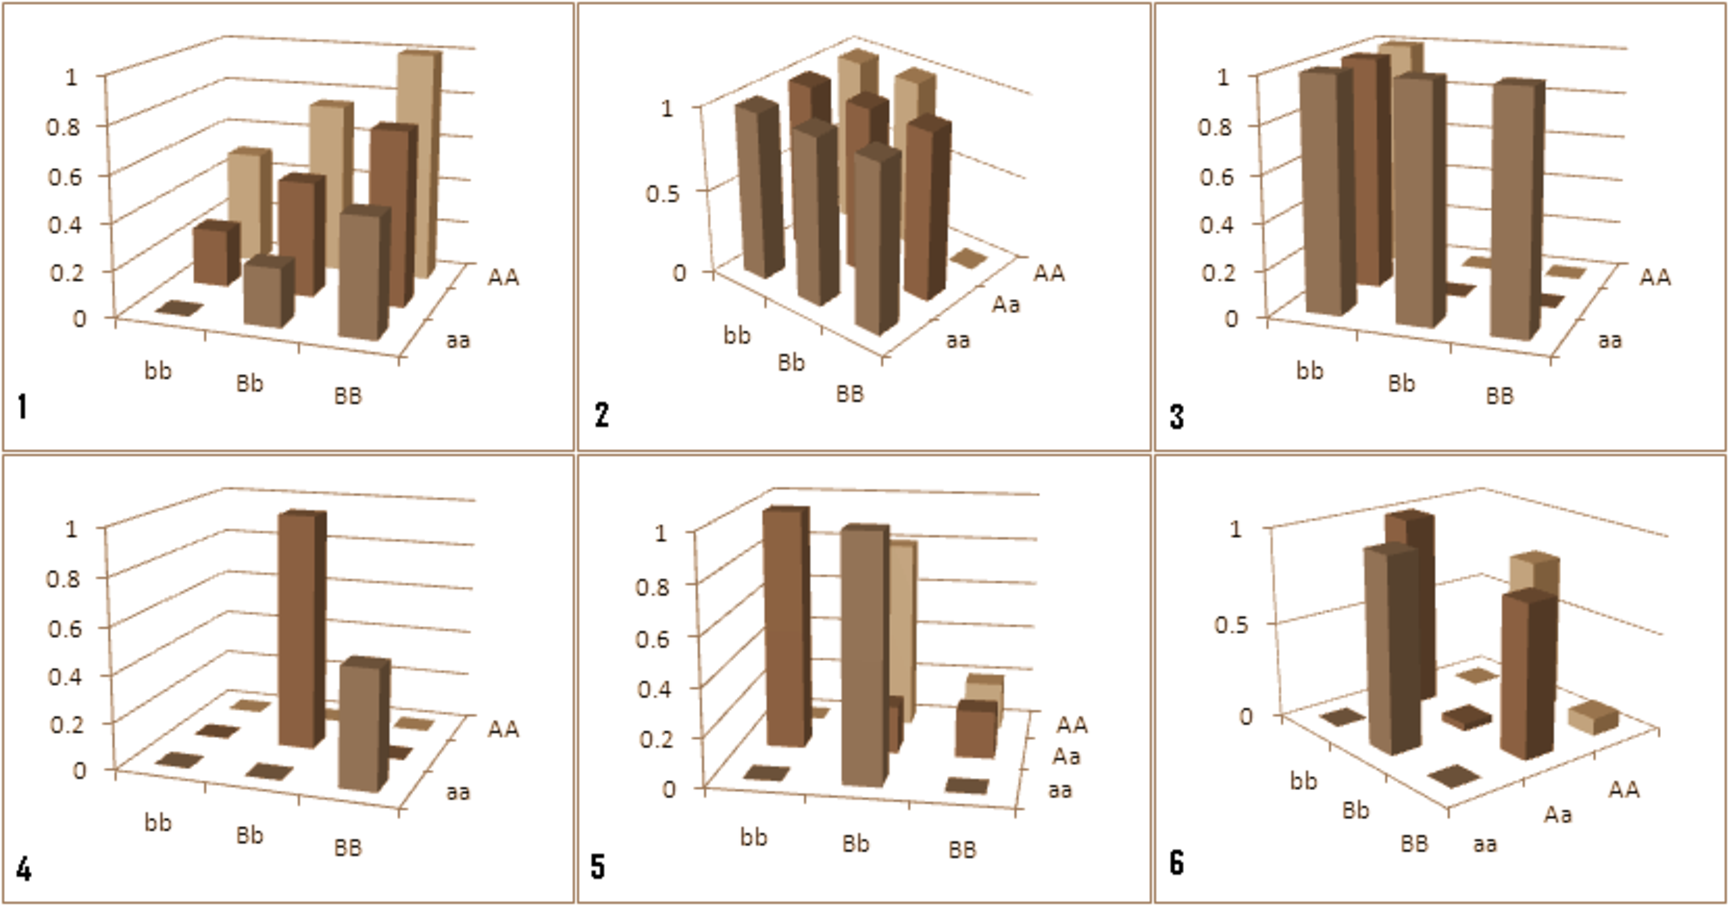
\includegraphics[width=8cm]{gpmaps2.pdf}
\end{center}
\end{frame}

\begin{frame}{Allele frequency trajectories}
\begin{center}
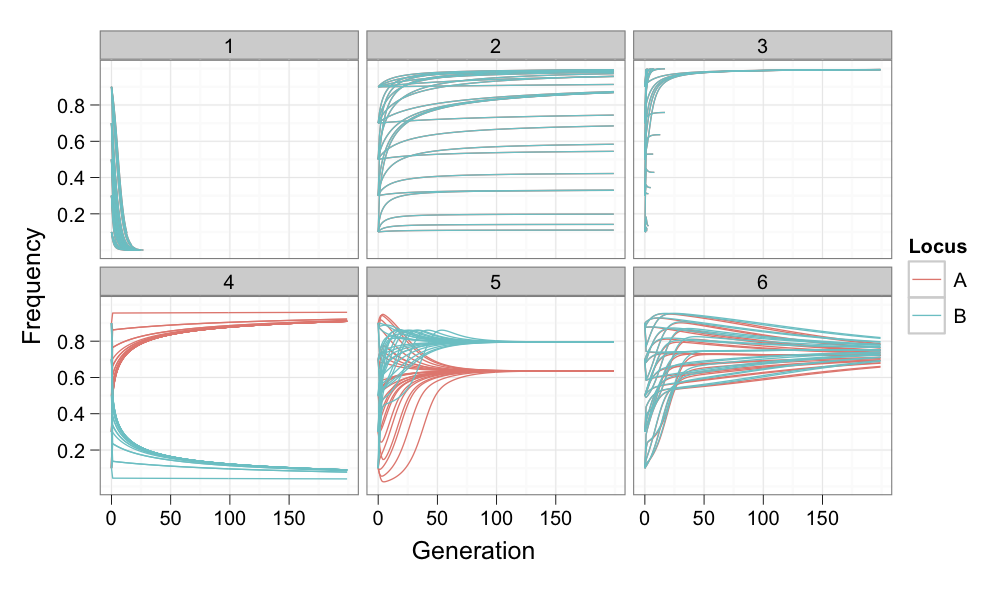
\includegraphics[width=8cm]{allelefreq_det.png}
\end{center}
\end{frame}

\begin{frame}{Changes in variance under selection}
\begin{center}
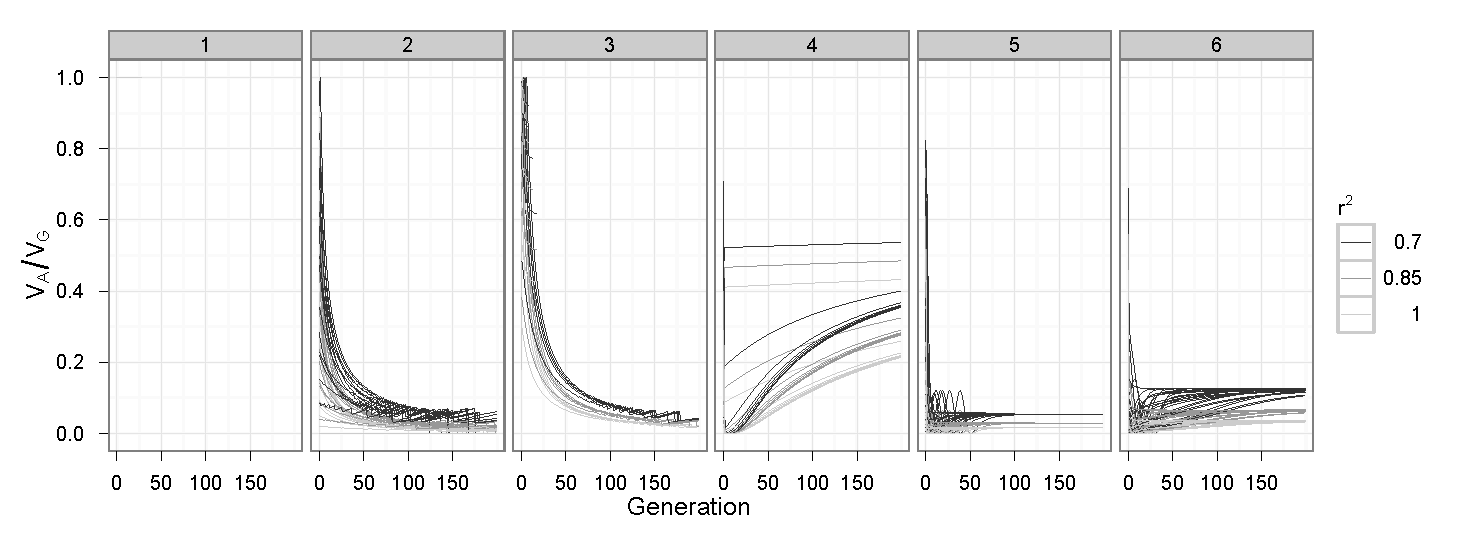
\includegraphics[width=10cm]{propadditive_det_grey.pdf} \\
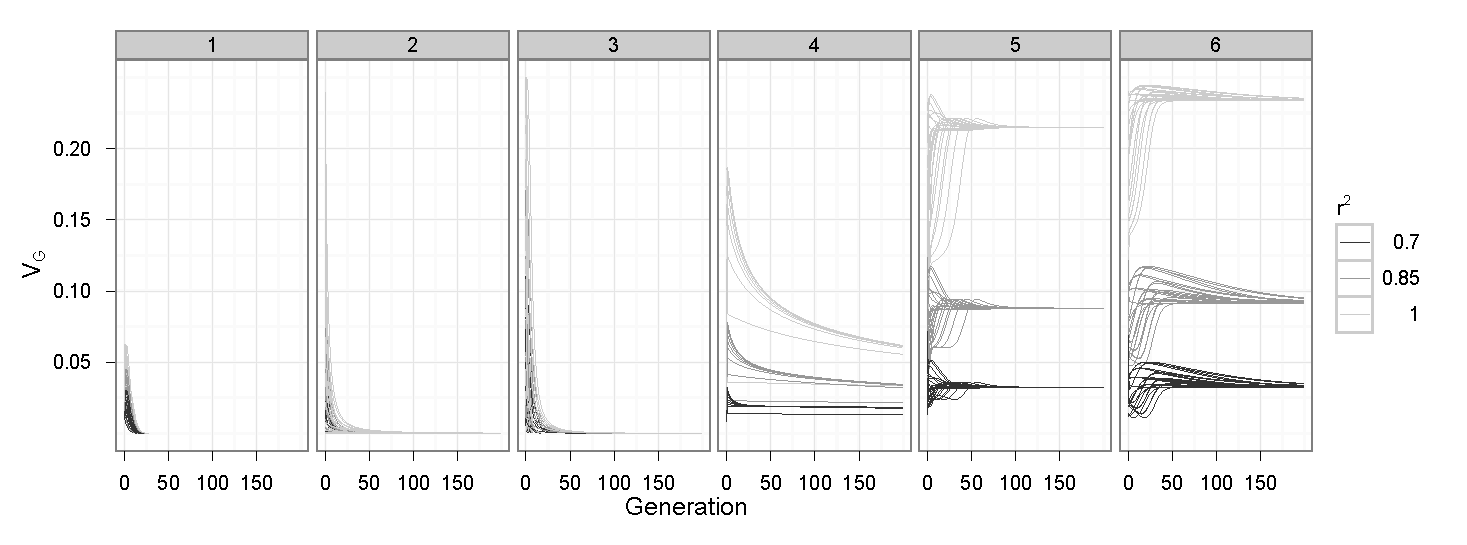
\includegraphics[width=10cm]{Vg_det_grey.pdf}
\end{center}
\end{frame}

\begin{frame}{Power studies}
\begin{center}
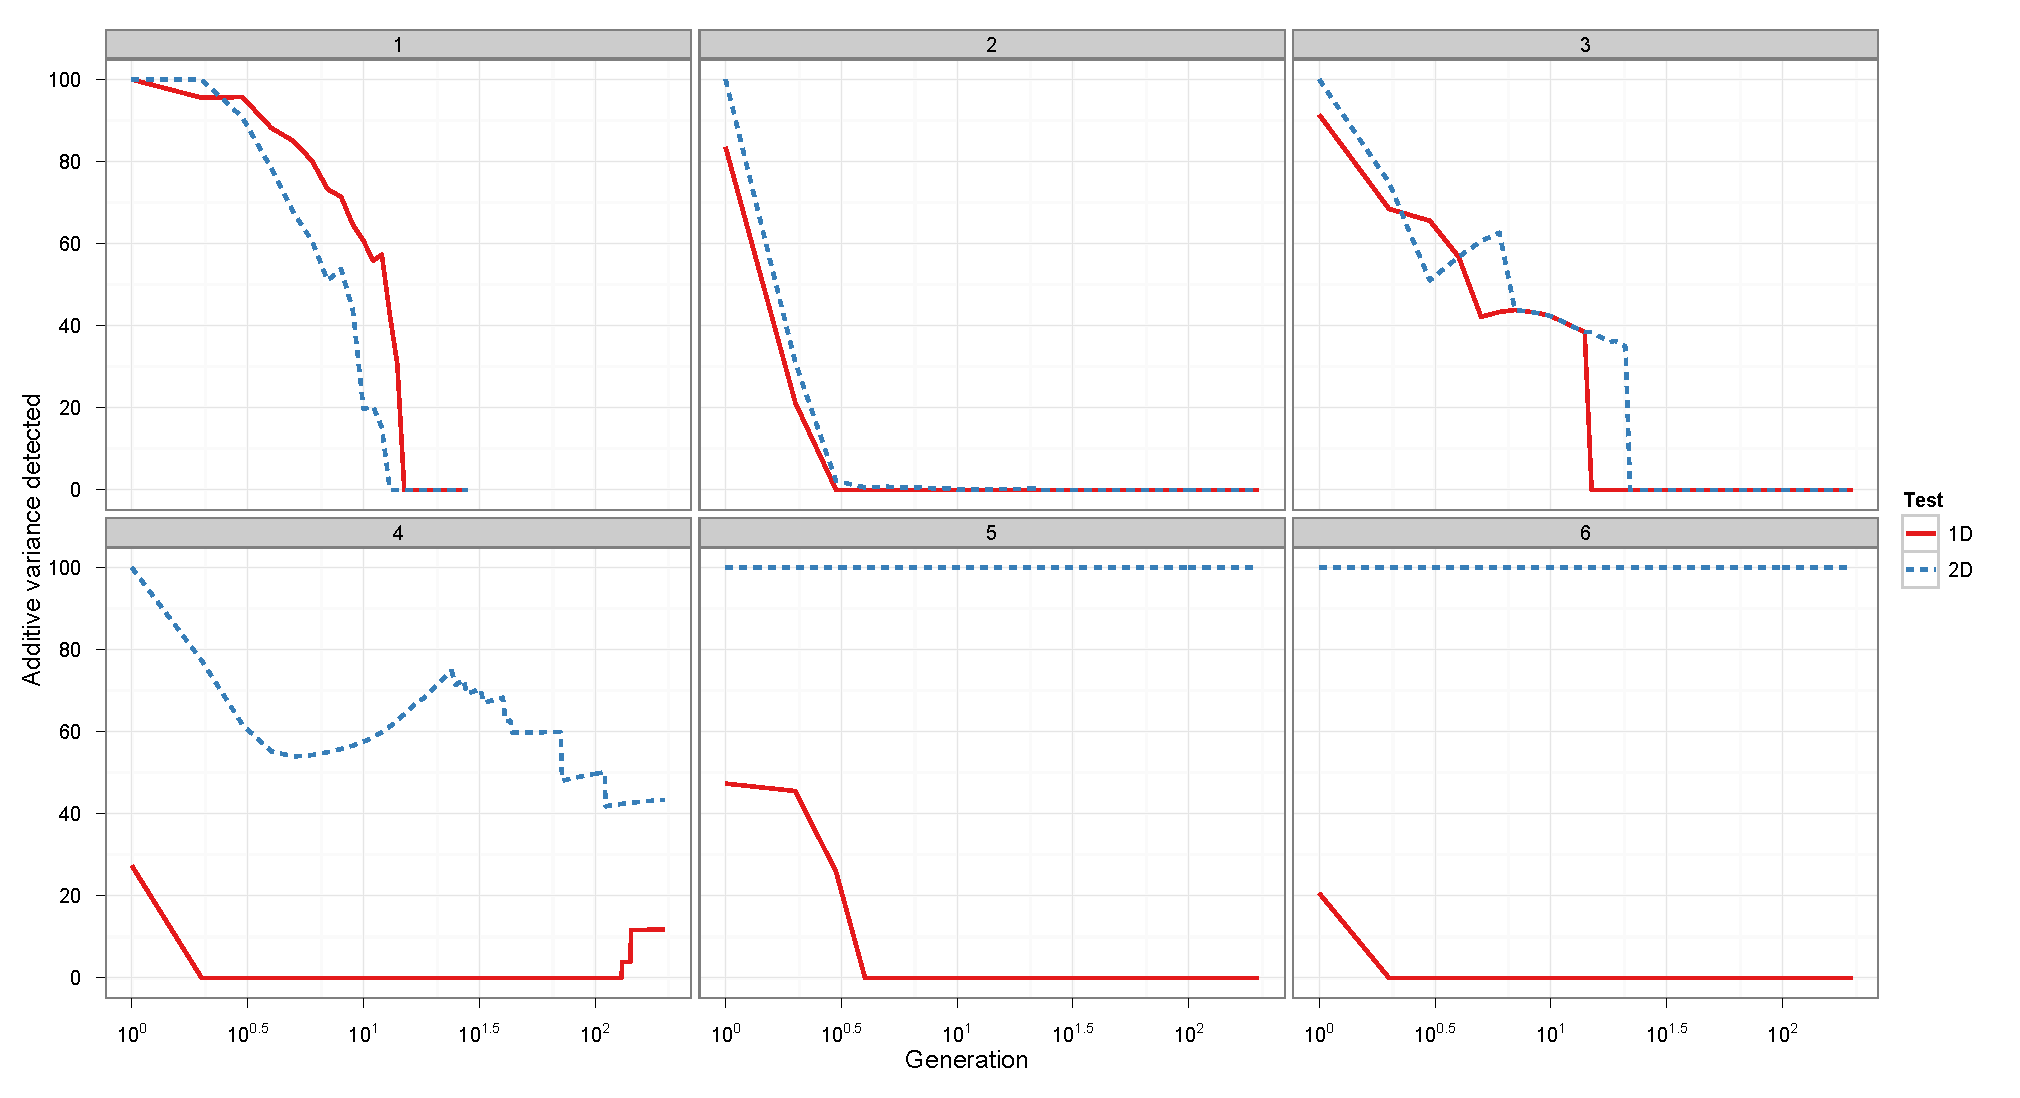
\includegraphics[width=10cm]{powersimple.pdf} \\
\end{center}
\end{frame}

\begin{frame}{Epistatic patterns}
\begin{center}
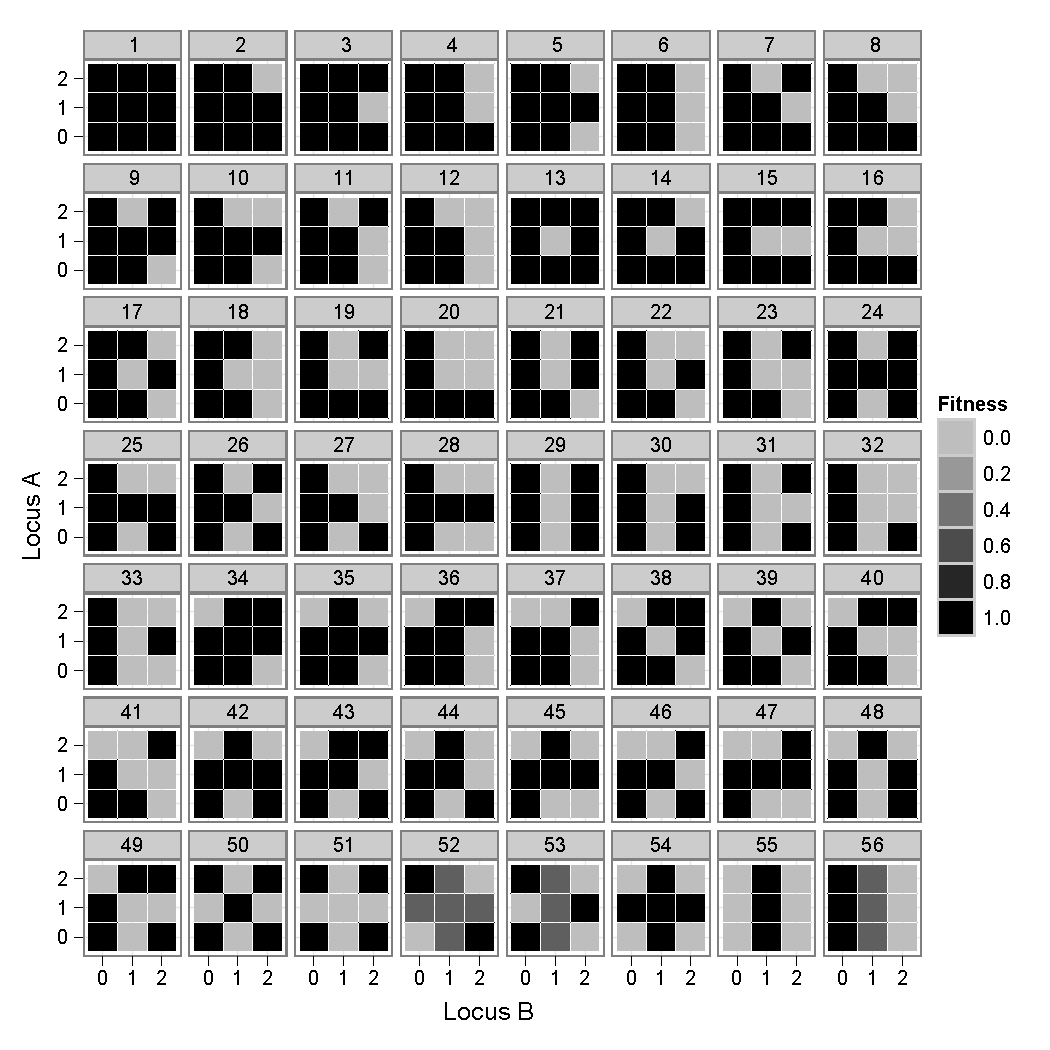
\includegraphics[width=8cm]{sup_gpmaps.pdf}
\end{center}
\end{frame}

\begin{frame}{Allele frequency trajectories}
\begin{center}
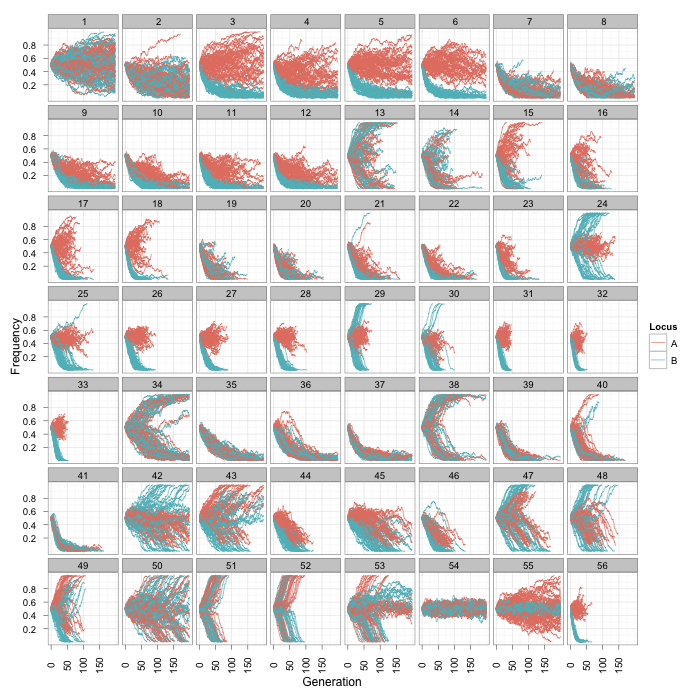
\includegraphics[width=8cm]{sup_allelefreq_sim.png}
\end{center}
\end{frame}


\end{document}


